\chapter{What actually happens, step by step}

\section{Turn the videos into pictures}

Sample a couple of frames per second, shrink them, and throw away the blurry ones. Blur is measured
by how sharp the edges are in the picture.

A blurry frame is worse than no frame at all, because the next stage works by recognising the same
corner in several different pictures, and blur destroys corners.

\section{Work out the shape of the room, from both videos at once}

\begin{watch}
This is the single most important decision in the project. If only one thing is remembered from
these notes, it should be this section.
\end{watch}

The obvious approach is to build a three dimensional model from video A, build a second one from
video B, and then line the two up.

That approach asks the hardest question first. Lining up two models works by finding the position
where they best agree, and it is least reliable exactly when part of the scene has genuinely moved.
The things that changed drag the alignment off, and once the alignment is wrong, everything looks
changed.

So instead, every frame from \textbf{both} videos goes into \textbf{one} reconstruction. The walls,
the floor and the furniture that stayed put appear in both recordings, so the software matches them
across the two videos by itself, and everything emerges in a single shared coordinate system. There
is no lining up step to get wrong.

\begin{plainbox}
Put simply: \textbf{the parts of the room that did not change are what tie the two visits
together}. The stable scene is the evidence. The changes are the thing being measured. Doing it the
other way round uses the unknown to establish the evidence.
\end{plainbox}

The code refuses to continue if both videos did not end up in the same model. A model containing
only video A would report the whole of video B as new, and that would look like a result rather
than a failure.

\section{Fill in the depth, and fix the scale}

The points from the previous step are accurate but sparse. Depth Anything fills in every pixel, but
its output has no scale.

The fix uses one against the other. Both describe the same frame, so finding the stretch and shift
that makes the estimated depths line up with the accurate sparse points converts the whole dense
estimate into the same units as the reconstruction. One small calculation per frame, and the dense
depth inherits whatever scale the reconstruction has.

Frames with too few sparse points to do this reliably are skipped rather than guessed at.

\begin{watch}
A wrongly scaled depth map does not produce a slightly wrong answer. It produces a confident answer
in completely the wrong part of the room, which is far more damaging than no answer.
\end{watch}

There is one further wrinkle. Reconstruction from photographs alone can never recover true
real-world size, because a doll's house photographed close up looks identical to a real house
photographed from further away. So the whole scene is rescaled once, so that typical distances come
out room sized. This is not true measurement, but it makes every setting in the configuration file
mean roughly what it appears to mean.

\section{Record what each visit knows, including what was empty}

Space is divided into a grid of cells, each five centimetres across. For each visit, every cell is
marked as one of three things.

\begin{center}
\begin{tabular}{@{}ll@{}}
\toprule
\textbf{Label} & \textbf{Meaning} \\
\midrule
occupied & something was measured here \\
free & a camera ray passed through here on its way to hitting something \\
 & further away, so this space was looked at and was empty \\
unknown & neither, so nothing can be said about it \\
\bottomrule
\end{tabular}
\end{center}

\textbf{Free is the state that makes this work.} Finding it means tracing the straight line from
the camera out to each thing it saw, and marking everything along the way as confirmed empty. It is
the most expensive part of the whole program and it is the reason the results can be trusted.

The tracing stops slightly short of the surface. Without that margin, the front face of every
object would erase itself and solid things would dissolve.

\section{Compare}

Two rules, and the whole argument of the project sits in them.

\begin{lstlisting}[language=,basicstyle=\ttfamily\small]
REMOVED  if occupied in visit A  AND  confirmed empty in visit B
ADDED    if occupied in visit B  AND  confirmed empty in visit A
\end{lstlisting}

Both require positive evidence from the other visit. A cell that held something in A and was simply
never looked at in B produces nothing at all, because nothing can honestly be claimed about it.

\begin{figure}[h]
\centering
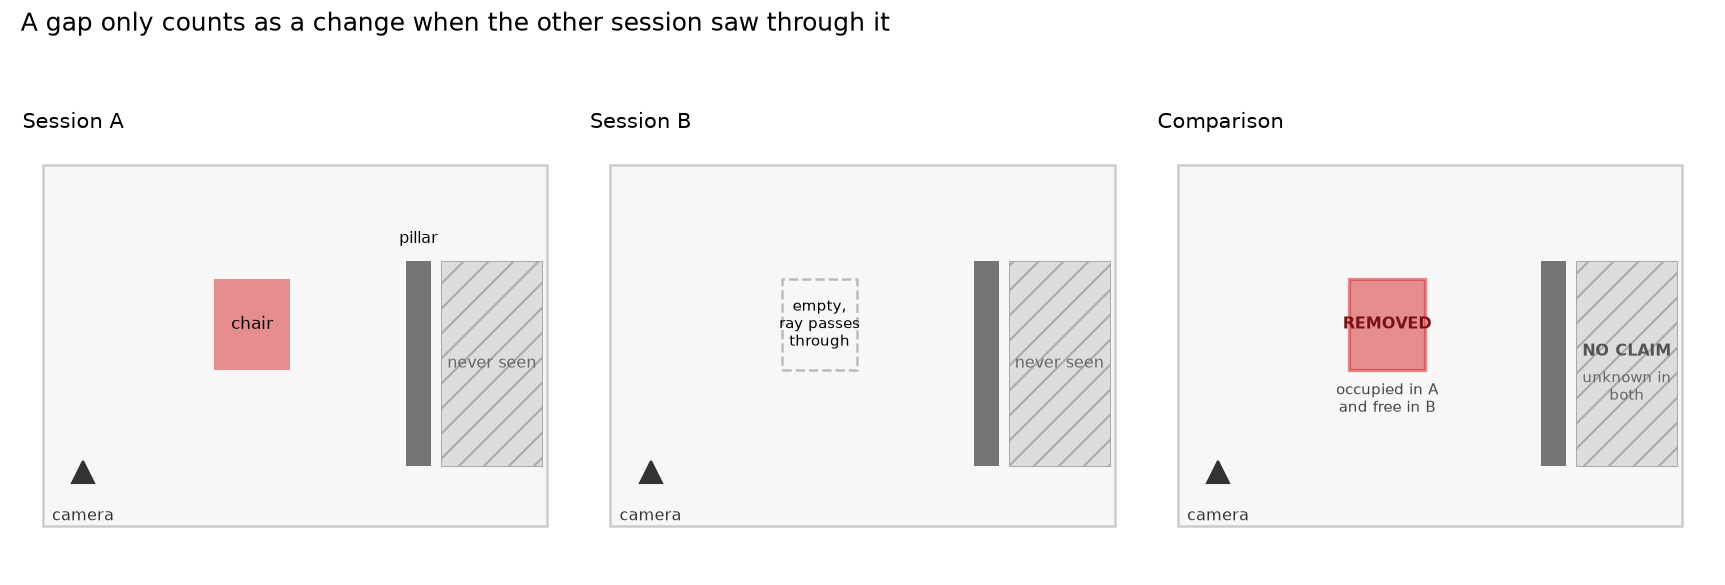
\includegraphics[width=\textwidth]{occupancy_states.png}
\caption{Why the third state matters. The chair is reported as removed because visit B positively
saw through that space. The region behind the pillar is not reported at all, because neither visit
could see it. A system that only tracked occupied space would report both as changes.}
\end{figure}

\begin{plainbox}
That one restriction is the difference between a system that reports \emph{what changed} and one
that reports \emph{where the camera went}.
\end{plainbox}

\section{Group, name, and pair up}

The changed cells are grouped into objects. Each group is then traced back into the photographs
that saw it, cropped out, and shown to CLIP for a name.

One subtle detail matters here. A removed object is cropped from a \textbf{visit A} photograph,
because by visit B it is not there any more.

\begin{watch}
Getting that backwards returns a picture of whatever is sitting in that space now, labels it
confidently, and produces output that is wrong while looking entirely reasonable. Those are the
worst kind of bugs, because nothing about the output announces the error.
\end{watch}

Finally, a disappearance in one place and an appearance in another are reported as a single
\textbf{move} only if they agree on name, are a similar size, and are not too far apart. Otherwise
they stay as two separate events, because that is the honest reading of the evidence.
